\newcommand\w[1]{\includegraphics[width=0.3\textwidth]{#1}}
\section{Representation}

\subsection{Diagrams}
\begin{frame}{\secname: \subsecname}
\note<1>[item]{let's look at some ways of representing string figures}
\note<1>[item]{we will start with a visual one, diagrams}

\pause Fingers are named $L1,\cdots, L5$ and $R1,\cdots,R5$ from thumb to pinky
\note<2>[item]{$L$ for left hand, $R$ for right hand}

\begin{itemize}
    \item \pause Ordered from nearest to furthest
    \note<3>[item]{i.e. order by the number}
    \pause \begin{center}
    $L1\lt L2\lt L3\lt L4\lt L5$\\
    $R1\lt R2\lt R3\lt R4\lt R5$    
    \end{center}
\end{itemize}

\pause String segments are named by finger $F\in\{L1,\cdots, L5,R1,\cdots,R5\}$
\begin{itemize}[<+(1)->]
    \item $Fn$ is the near string, $Ff$ is the far string
    \item $Lp$ and $Rp$ are palmar strings
\note<.(1)>[item]{ when we have a string between $L1$ and $L5$, we give a special name, called palmar string}
\end{itemize}
\end{frame}

\begin{frame}{\secname: \subsecname}
\includegraphics[width=0.9\columnwidth]{figures/open.png}
% \begin{figure}\centering
% \def\svgwidth{0.9\columnwidth}
% \input{figures/open.pdf_tex}
% \end{figure}
\end{frame}
\note[itemize]{
\item an actual diagram would look like this
\item top down view of the fingers
\item write segments, write $Lp$
\item ARE WE OK WITH THIS???
\item ...
\item the diagrams are intuitive and very visual, but they are less computer friendly
\item what do computers like? they like array of symbols
}

\subsection{Linear Sequences}
\begin{frame}{\secname: \subsecname}
Two components
\begin{itemize}[<+(1)->]
    \item Fingers that hold the string
    \item Crossings between two segments
\end{itemize}

\pause Diagram $\to$ linear sequence

\begin{itemize}[<+(1)->]
    \item Start with left nearest finger and travel clockwise
    \item Visit fingers and crossings
\end{itemize}

\note<5>[item]{travel along the string clockwise}
\note<6>[item]{we would write down the fingers and crossings to make a linear sequence}
\end{frame}

\begin{frame}{\secname: \subsecname}
\begin{center}
    \includegraphics[width=0.7\columnwidth]{figures/open.png}
\end{center}
$$L1:L5:R2$$
\end{frame}
\note[itemize]{
\item an algorithm that converts diagrams to linear sequences would map this to $L1:R5:R2$
\item ARE WE OK WITH THIS
}

\begin{frame}[t]{Linear Sequences with Crossings}
Diagram $\to$ linear sequence
\note<1>[item]{what do we do if we see crossings}
\begin{itemize}[<+(1)->]
    \item Name each crossing as $x_i$ for some $i$
    \item Visit overcrossing $\implies$ write $x_i(o)$
    \item Visit undercrossing $\implies$ write $x_i(u)$
\end{itemize}

\end{frame}

\note[itemize]{
\item draw overcrossing and undercrossing
}


\begin{frame}{Linear Sequences with Crossings}
\begin{adjustwidth}{-1.5em}{-1.5em}
\begin{center}
\includegraphics[width=0.7\columnwidth]{figures/star-pick.png}
\end{center}

$$
L1:x_2(o):R5:x_1(o):L5:x_1(u):x_2(u):R2
$$
\end{adjustwidth}
\end{frame}

\note[itemize]{
\item if we have $n$ fingers holding the string figure that has $m$ crossings, the sequence will have $n+2m$ symbols
\item in this case we have $4$ fingers and $2$ crossings, so the sequence is $4+2*2=8$ symbols long
\item in most cases, we are making more and more crossings in each step, so it would be tedious to write down the entire sequence by hand
\item which gives us more motivation to develop a systematic way of computing the movements so we can let computer do the calculation
\item ...
\item the most common movements involve a finger and a near/far string segment
\item eg this string figure is made from the opening with pick on $Lp$
\item so if we want to pick $Lp$ on the linear sequence, we need to first identify the segment from the sequence alone
}


\subsection{Identifying String Segments }

\begin{frame}{\subsecname from Linear Sequences}
\begin{adjustwidth}{-1.5em}{-1.5em}
Consider a left-hand finger $L_i$ in the sequence

\begin{itemize}[<+(1)->]
    \item Traverse clockwise \raisebox{-0.45\height}{\includegraphics[width=0.2\textwidth]{figures/leftcw.png}} \pause $\implies \ldots:[n] L_i [f]:\ldots$
    \item Traverse counterclockwise \raisebox{-0.45\height}{\includegraphics[width=0.2\textwidth]{figures/leftccw.png}} \pause $\implies\ldots: [f] L_i [n]:\ldots$
\end{itemize}

\pause Similarly for finger $R_i$ on the right hand

\begin{itemize}
    \item \raisebox{-0.45\height}{\includegraphics[width=0.2\textwidth]{figures/rightcw.png}} $\implies \ldots:[f]R_i[n]:\ldots$
    \item\raisebox{-0.45\height}{\includegraphics[width=0.2\textwidth]{figures/rightccw.png}} $\implies\ldots:[n]R_i[f]:\ldots$
\end{itemize}
\end{adjustwidth}
\end{frame}

\note[itemize]{
\item ...
\item since we always start a linear sequence by going clockwise, we can figure the segments on the first finger
\item how about other fingers
}

\begin{frame}{\subsecname: Opposite Hand}
\begin{adjustwidth}{-1.5em}{-1.5em}
Consider $\ldots:L_i:\ldots:R_j:\ldots$
\note<1>[item]{suppose the next finger is on the opposite hand}
\begin{itemize}[<+(1)->]
    \item Even number of crossings between $L_i$ and $R_j\implies$ orientation persists\\
    \begin{center}
    \includegraphics[width=0.5\columnwidth]{figures/diff-even.png}
    $$
    [n]L_i[f]:[f]R_j[n]
    $$
    \end{center}
    \item Odd number of crossings between $L_i$ and $R_j\implies$ orientation reverses\\
    \begin{center}
    \includegraphics[width=0.5\columnwidth]{figures/diff-odd.png}
    $$
    [n]L_i[f]:x_1(u):[n]R_j[f]:x_1(o)
    $$
    \end{center}
\end{itemize}
\end{adjustwidth}
\end{frame}
\note[itemize]{
\item write $x_1$
\item show 2 crossings: twist twice
}

\begin{frame}{\subsecname: Same Hand}
\begin{adjustwidth}{-1.5em}{-1.5em}
Consider $\ldots:L_i:\ldots:L_j:\ldots$

\vfill
\pause
\begin{minipage}{0.5\textwidth}
\begin{center}
Even $\implies$ orientation persists\\
\includegraphics[width=0.3\linewidth]{figures/same-even.png}
\end{center}
$$
\scriptstyle
\ldots:[n]L_i[f]:[n]L_j[f]:\ldots
$$
\end{minipage}
\hfill
\pause
\begin{minipage}{0.5\textwidth}
\begin{center}
Odd $\implies$ orientation reverses\\
\includegraphics[width=0.3\linewidth]{figures/same-odd.png}
\end{center}
$$
\scriptstyle
\ldots:[n]L_i[f]:x_1(u):[f]L_j[n]:x_1(o):\ldots
$$
\end{minipage}
\end{adjustwidth}
\end{frame}

\begin{frame}[t]{\subsecname: Example}

$$
{L1}:x_2(o):R5:x_1(o):L5:x_1(u):x_2(u):R2
$$

\pause {By convention, the first finger in the linear sequence is clockwise}

\begin{adjustwidth}{-2em}{-2em}
$$
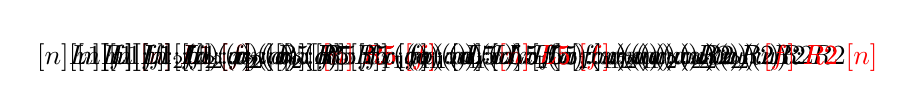
\begin{tikzpicture}
    \node<+> at(0,0){$\stackrel{\phantom\curvearrowright}{L1}:x_2(o):R5:x_1(o):L5:x_1(u):x_2(u):R2$};
    \node<+> at(0,0){${\color{red}\stackrel\curvearrowright{L1}}:x_2(o):R5:x_1(o):L5:x_1(u):x_2(u):R2$};
    \node<+> at(0,0){${\color{red}[n]\stackrel\curvearrowright{L1}[f]}:x_2(o):R5:x_1(o):L5:x_1(u):x_2(u):R2$};
    \node<+> at(0,0){$[n]\stackrel\curvearrowright{L1}[f]:x_2(o):{\color{red}\stackrel\curvearrowleft{R5}}:x_1(o):L5:x_1(u):x_2(u):R2$};
    \node<+> at(0,0){$[n]\stackrel\curvearrowright{L1}[f]:x_2(o):{\color{red}[n]\stackrel\curvearrowleft{R5}[f]}:x_1(o):L5:x_1(u):x_2(u):R2$};
    \node<+> at(0,0){$[n]L1[f]:x_2(o):[n]\stackrel\curvearrowleft{R5}[f]:x_1(o):{\color{red}\stackrel\curvearrowright{L5}}:x_1(u):x_2(u):R2$};
    \node<+> at(0,0){$[n]L1[f]:x_2(o):[n]\stackrel\curvearrowleft{R5}[f]:x_1(o):{\color{red}[n]\stackrel\curvearrowright{L5}[f]}:x_1(u):x_2(u):R2$};
    \node<+> at(0,0){$[n]L1[f]:x_2(o):[n]R5[f]:x_1(o):[n]\stackrel\curvearrowright{L5}[f]:x_1(u):x_2(u):{\color{red}\stackrel\curvearrowright{R2}}$};
    \node<+> at(0,0){$[n]L1[f]:x_2(o):[n]R5[f]:x_1(o):[n]\stackrel\curvearrowright{L5}[f]:x_1(u):x_2(u):{\color{red}[f]\stackrel\curvearrowright{R2}[n]}$};
\end{tikzpicture}
$$
\end{adjustwidth}

$$\begin{tikzpicture}
    \node<3>at(0,0){\w{figures/leftcw.png}};
    \node<5>at(0,0){\w{figures/rightccw.png}};
    \node<7>at(0,0){\w{figures/leftcw.png}};
    \node<9>at(0,0){\w{figures/rightcw.png}};
\end{tikzpicture}$$
\end{frame}

\begin{frame}{\subsecname: Example}
$$
[n]L1[f]:x_2(o):[n]R5[f]:x_1(o):[n]{L5}[f]:x_1(u):x_2(u):{[f]{R2}[n]}
$$

\begin{center}
\includegraphics[width=0.7\columnwidth]{figures/star-pick.png}
\end{center}
\end{frame}

\note[itemize]{
\item trace sequence
\item ARE WE OK WITH THIS
\item the the point is that once we get a linear sequence, we can identify the segments without diagrams
\item so when want to pick a specific string segment, we know where it is in the linear sequence
\item (draw $L1:L5:R2$)
\item so to do "pick $Lp$ with $R5$", we need to first identify where $Lp$ is in the sequence, and insert $R5$ there with some crossings
\item ...
\item to describe picking, we need to define another simpler movement first, which is twisting
}